\chapter{Introdución}
\label{chap:introducion}

\lettrine{E}{l} uso de prótesis a falta de miembros en el cuerpo es una historia que nos persigue desde antes de Cristo, debido a las limitaciones de la época estamos hablando de implantaciones fijas sin ningún tipo de utilidad que lo largo de los años y con ayuda de los avances en electrónica y mecánica el ser humano ha sido capaz de mejorar. Actualmente, existen prótesis avanzadas que son capaces de devolver al paciente una importante variedad de movimientos. Aun así, debido a factores como el mercado de producción o la tecnología nos encontramos con productos que no están a la disposición de cualquiera, la relación precio/utilidad está muy presente en la vida de los amputados.\\

En cuanto a la facilidad que hay para acceder a herramientas de desarrollo en este tipo de proyectos en concreto, ya sean, elementos Hardware de sensorización, conversión analógico digital y Software especializado, fue difícil encontrar una plataforma con la que poder trabajar fácilmente y por poco precio. Este TFG tiene también como objetivo ayudar a identificar las mejores opciones y ofrecer herramientas de tipo Open Source que se puedan utilizar por cualquiera.\\

Para llegar a conseguir que las prótesis electromecánicas sean asequibles y llamativas de convertirse en un producto es interesante también analizar otros usos que se le puede dar y se le está dando a esta tecnología. Entre más utilizada sea, mayor mercado se creará, menores serán los costes, mejor será la competencia y en definitiva los productos verán aumentada su calidad. 
Este análisis de mercado se basará entonces en el concepto de que con la electromiografía, buscamos extraer información de la actividad actividad muscular para con ella reconocer patrones de movimientos e incluso extraer características de cada músculo implicado, por esto mismo descubrí que actualmente se empieza a ver aplicada en la fisioterapia como herramienta para la valoración muscular y del ejercicio en clientes.
La empresa española MDURANCE se encarga de suministrar este tipo de equipamiento para clínicas y ha conseguido una buena recepción entre sus compradores, ofreciendo tanto Hardware como Software listo para usar por los fisioterapeutas en sus sesiones.

\begin{figure}[hp!]
\begin{center}
    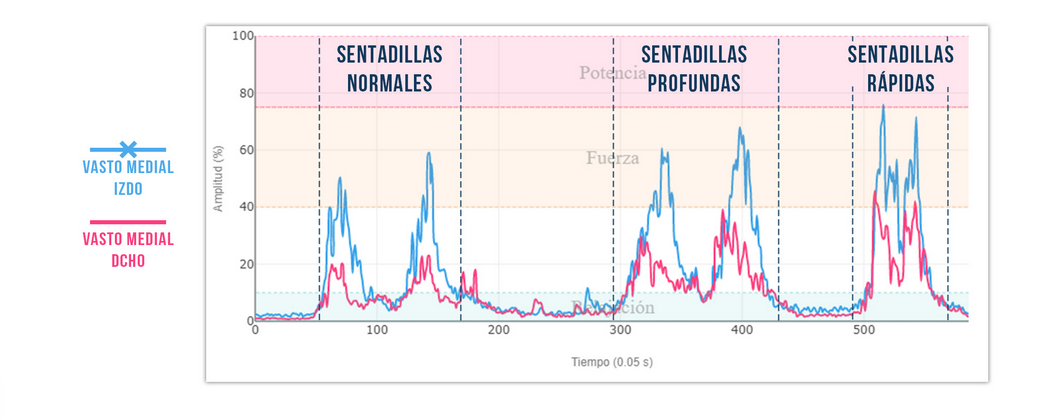
\includegraphics[width=1\textwidth]{imaxes/mdurance1.png}
    \caption{ActionButton}
    
    \vspace{1cm}

    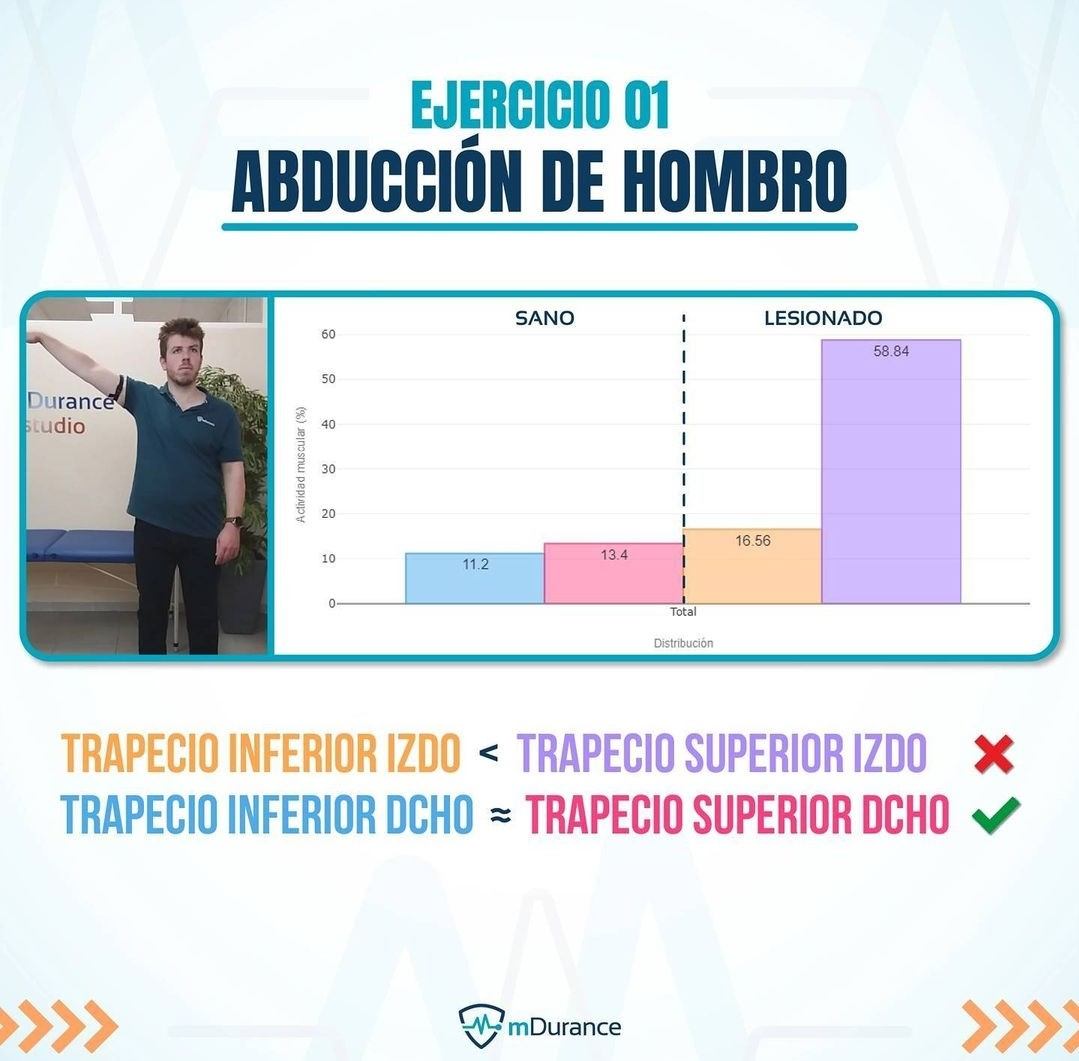
\includegraphics[width=0.75\textwidth]{imaxes/mdurance2.jpg}
   \vspace{0.1cm}
    \caption{ActionButton}
    \label{ActionButton}
  \end{center}
\end{figure}



Como se puede ver, este tipo de herramienta es utilizada para obtener lecturas de la actividad muscular durante ciertos movimientos y así ofrecer al especialista información más detallada e individual sobre sinergias musculares, descompensaciones, fatiga... 
Lo que más me parece interesante sobre el producto que ofrecen en MDURANCE es la escalabidad que tiene para implementar un sistema que no solo se base en la electromiográfia y pueda crecer hacia un asistente clínico que tenga capacidad de sacar conclusiones en base a diferentes datos que recolecta durante las sesiones. Ahora mismo, cuentan también con videofeedback y monitorización del progreso. 

Otro uso interesante que se podría ver en el mercado de la electromiografía se encuentra en las interfaces hombre-máquina, donde se podría utilizar como método para controlar elementos externos mediante la caracterización de movimientos. Un ejemplo sencillo se encontraría dentro de la Realidad Virtual, en donde se busca sumergir a la persona en un mundo completamente digital, donde existe un avatar controlado por los movimientos de la misma. Y no solo eso, los juegos también son un método interesante para introducir a la gente en este tipo de tecnologías y hacer más amigable la interacción durante los experimentos para así, enseñar de forma gráfica y divertida de que se trata. A parte de esto, también se puede pensar en utilizarlo para controlar cualquier tipo de máquina.\\

\begin{figure}[!h]
  \centering
  \begin{tabular}[c]{cc}
    \begin{subfigure}[c]{0.5\textwidth}
      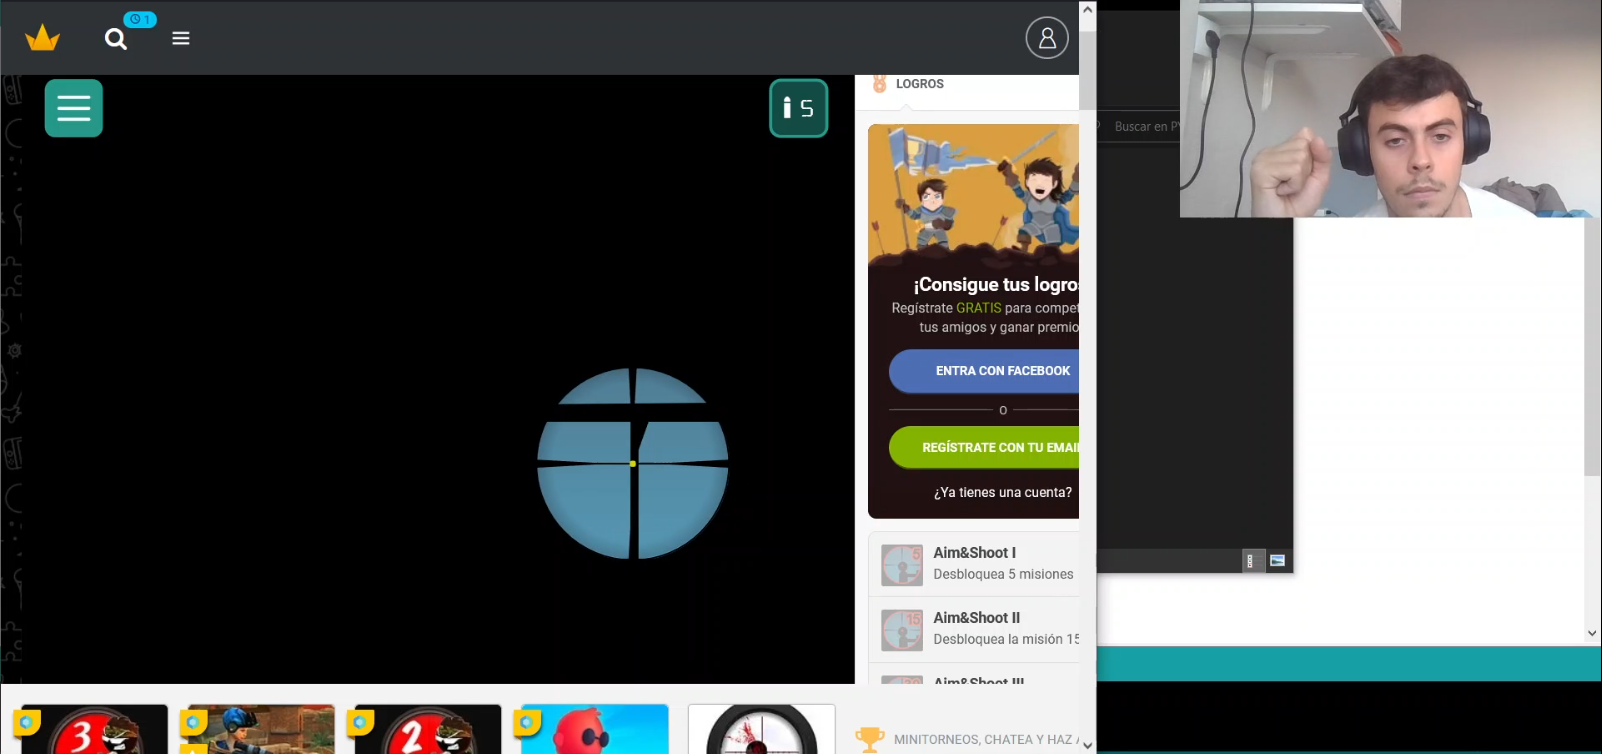
\includegraphics[width=\textwidth]{imaxes/juego1.png}
      
    \end{subfigure}&
    \begin{subfigure}[c]{0.5\textwidth}
      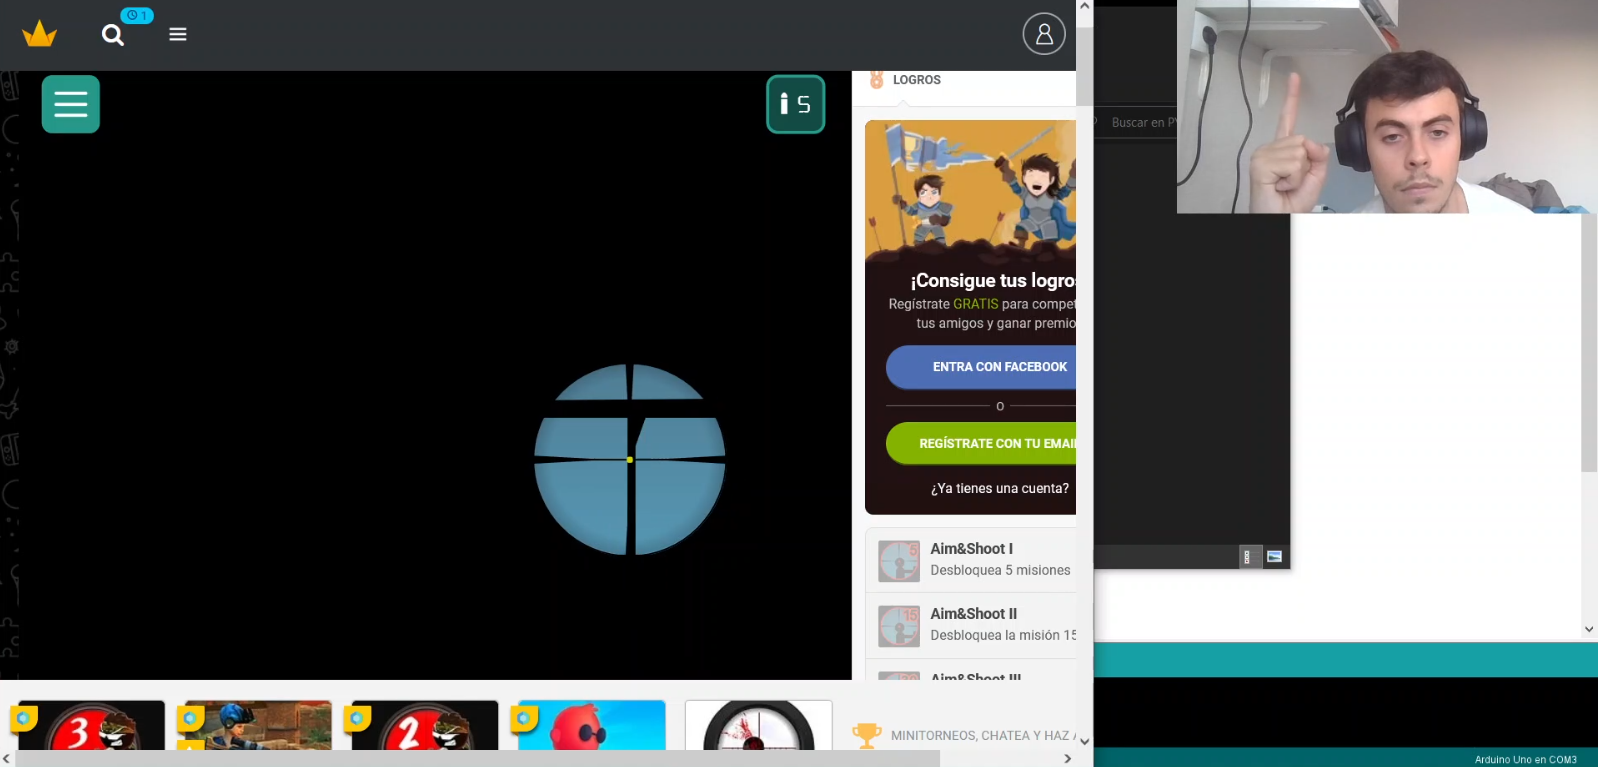
\includegraphics[width=\textwidth]{imaxes/juego2.png}
      
      
    \end{subfigure}\\
    \begin{subfigure}[c]{0.5\textwidth}
      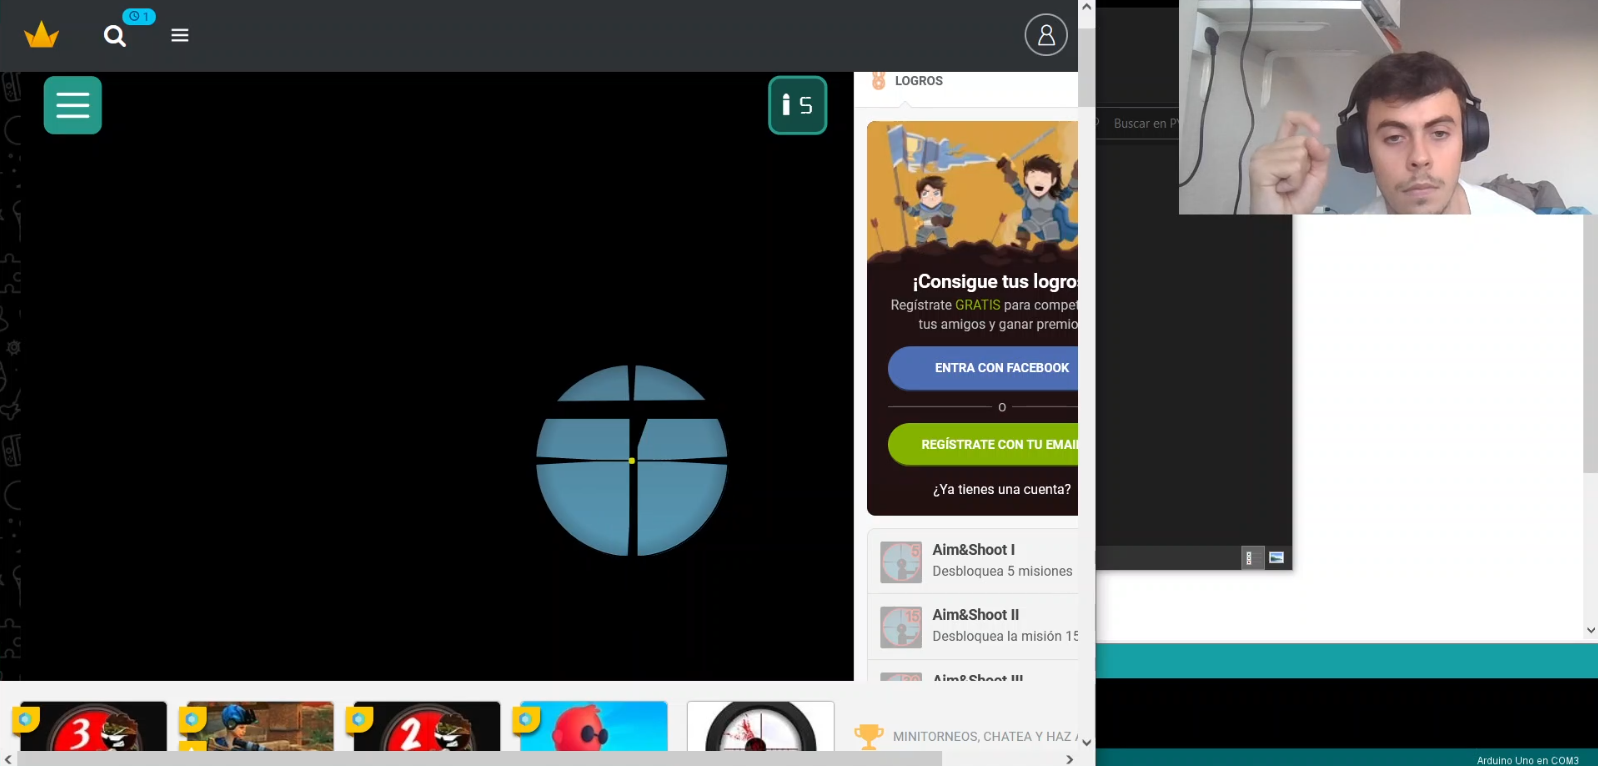
\includegraphics[width=\textwidth]{imaxes/juego3.png}
      
    \end{subfigure}&
    \begin{subfigure}[c]{0.5\textwidth}
      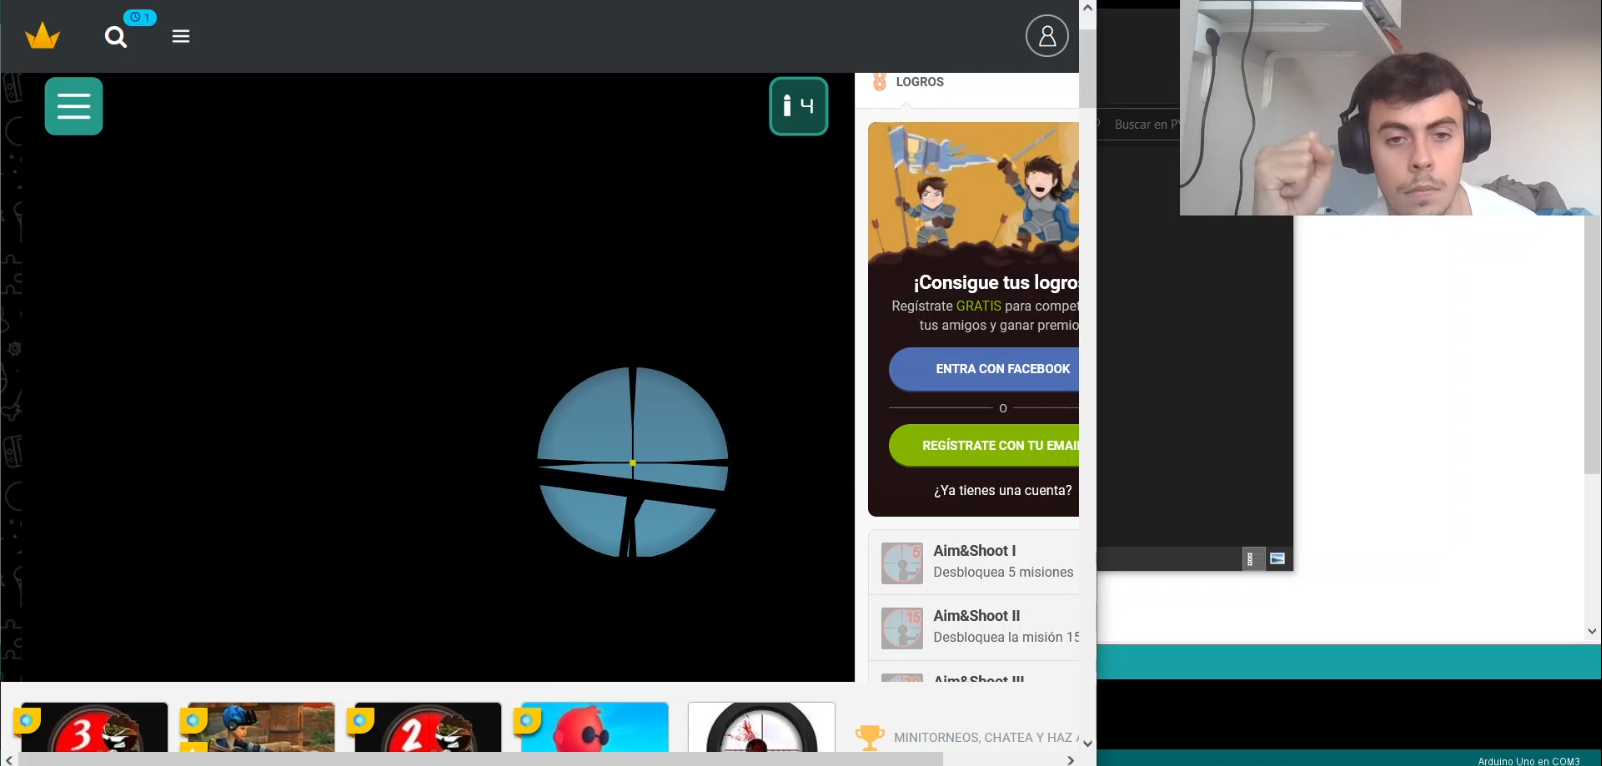
\includegraphics[width=\textwidth]{imaxes/juego4.png}
      
    \end{subfigure}\\
  \end{tabular}    
 
\end{figure}


\section{Anatomía básica y lectura de señales}
\label{sec:mostra}

Los músculos son un tipo de tejido blando que puede contraerse mediante impulsos nerviosos, generando movimiento y permitiendo trabajos mecánicos. La electromiografía es una técnica que mide la actividad eléctrica generada por el paso del impulso nervioso, que provoca la despolarización de la membrana de la célula muscular durante la excitación. Si la despolarización alcanza un determinado valor umbral, se genera un potencial de acción.\\

\begin{figure}[hp!]
\begin{center}
    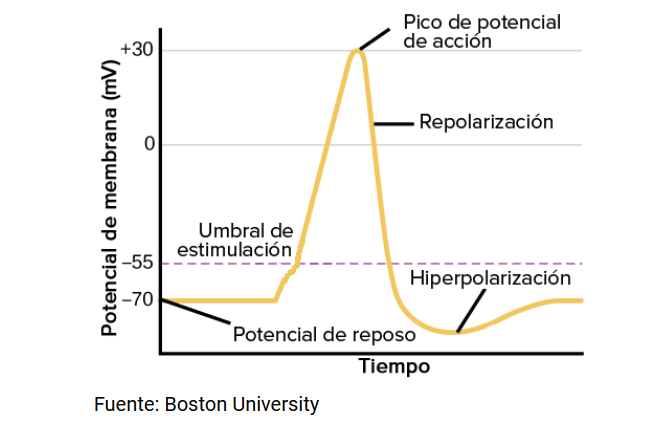
\includegraphics[width=1\textwidth]{imaxes/emg.png}
    \caption{ActionButton}
    
    \vspace{1cm}

    \label{ActionButton}
  \end{center}
\end{figure}


Para las mediciones, comúnmente se hace uso de dos emisores (uno en cada extremo del musculo a medir) y un GND (normalmente ubicado en zona de hueso) para extraer una señal mas limpia que posteriormente se amplifica y filtra. Son también llamamos electrodos y existen diferentes tipos de los mismos en los que podemos diferenciar los pasivos, activos, húmedos o en seco. Sobre ellos creo que actualmente los más cómodos de utilizar los secos, ya que permiten una fácil interacción y se pueden recolocar facilmente, igualmente pienso en que habría que reinventar un poco el formato en el que se utilizan.

Por tanto, la EMG mide de una manera indirecta la actividad muscular, ya que es capaz de determinar si el sistema nervioso está reclutando activamente un músculo durante una tarea específica.(MDURANCE)\\

Aplicado al control de prótesis es importante reconocer y estudiar las zonas de donde se van a tomar las lecturas, dependerá del tipo de amputación, del numero de señales que queramos usar para el control e incluso de características como el porcentaje de grasa que tiene el paciente en cuerpo, la edad.. En nuestro caso al tratarse de una prótesis de 2 canales mediremos la actividad del flexor carpi radialis y el extensor carpi radialis longus. Estos músculos ubicados en el antebrazo están implicados en varios movimientos de la mano, el flexor carpi tiene la acción de flexor principal de la muñeca, con tendencia a su abducción y pronación. También es flexor del codo. El otro, en la articulación del codo realiza ligera flexión y en la de la muñeca extensión colaborando en el cierre del puño y desviación radial.\\ 

De esta zona podríamos diferenciar señales incluso provenientes de cada dedo por individual, pero ello implicaría mayor y mejor sensorización y una capacidad de inteligencia superior en el controlador para diferenciar las señales provenientes de cada movimiento, esto sería lo mas interesante si queremos imitar al máximo el comportamiento de una mano pero tendría ciertas restricciones como el aumento del costo, un periodo mayor de adaptación y entrenamiento para el paciente e incluso un incremento en el tamaño o en el peso de la implantación. Lo que busco en este proyecto, es desarrollar un sistema funcional al precio mas bajo que sea capaz de conseguir, adelantando ya que es posible conseguir muy buenos resultados a bajo coste.

\begin{figure}[hp!]
\begin{center}
    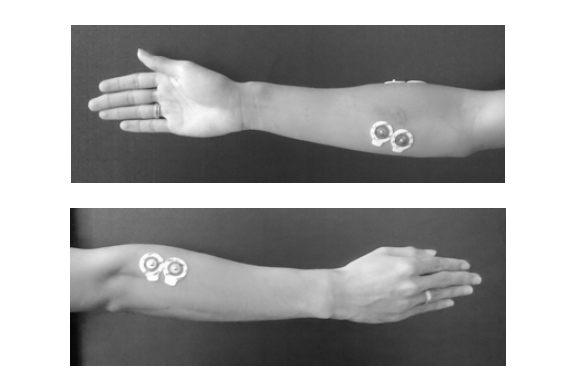
\includegraphics[width=0.75\textwidth]{imaxes/electrodos.png}
    \caption{ActionButton}
    
    \vspace{1cm}

    \label{ActionButton}
  \end{center}
\end{figure}



%\subsection{Subsección de mostra}
%\Blindtext
